\documentclass[tikz,border=10pt]{standalone}
\begin{document}
% definition of the pieces, just to show that in
% both configurations the same ones are used
\newcommand{\bluetriangle}[1][]{
  \draw[fill=blue,#1]
       (0,0)--( 8,0)--( 8,3)--cycle;}
\newcommand{\yellowtriangle}[1][]{
  \draw[fill=yellow,#1]
       (8,3)--(13,3)--(13,5)--cycle;}
\newcommand{\redpolygon}[1][]{
  \draw[fill=red,#1]
       (8,0)--(13,0)--(13,2)--(10,2)--(10,1)--(8,1)--cycle;}
\newcommand{\greenpolygon}[1][]{
  \draw[fill=green,#1]
       (8,1)--(10,1)--(10,2)--(13,2)--(13,3)--(8,3)--cycle;}
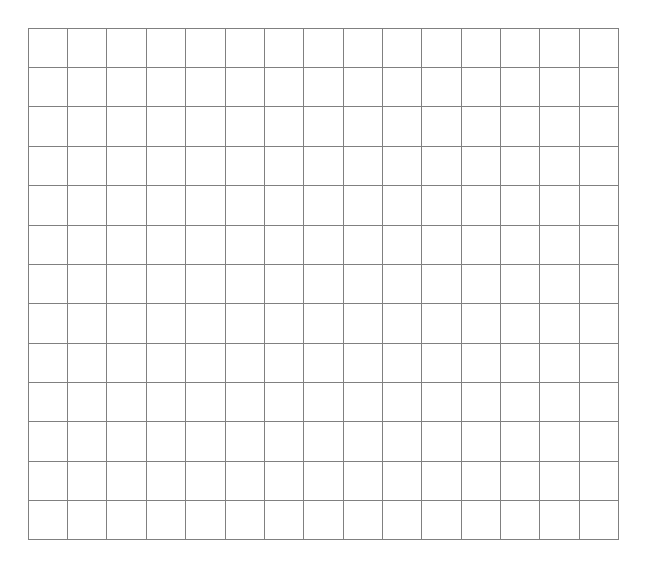
\begin{tikzpicture}[x=0.5cm,y=0.5cm,thick]
% the grid
  \draw[help lines,step=1] (-1,-1) grid (14,12);
% the complete triangle
    \bluetriangle
    \yellowtriangle
    \redpolygon
    \greenpolygon
% the missing square triangle
  \begin{scope}[yshift=3cm]
    \bluetriangle  [shift={( 5, 2)}]
    \yellowtriangle[shift={(-8,-3)}]
    \redpolygon    [shift={( 0, 0)}]
    \greenpolygon  [shift={(-3,-1)}]
  \end{scope}
% the solution (uncomment next line and close in)
%    \draw[very thin,red] (0,0)--(13,5) {[yshift=3cm] (0,0)--(13,5)};
\end{tikzpicture}
\end{document}
